\section{Experimental Results}

\begin{frame}{Experimental Results}
	\begin{table}[]
		\scriptsize
		\centering
		\begin{tabular}{crccr}
			  & Size    & File  & Directory & Merkle tree Size \\
			  &			&		&		    &                  \\
			A & 777 MB  & 48    & 6         & 5.4 KB           \\
			B & 145 MB  & 54198 & 188       & 5.08 MB          \\
			C & 5.95 GB & 45089 & 1459      & 4.37 MB          \\
		\end{tabular}
        
		\caption{GENERATE MERKLE TREE'S TIME (IN SEC.)}
		\begin{tabular}{|c|r|c|c|c|}
			\hline
			   &             & A      & B       & C       \\ \hline
               &             &        &		    &		  \\ \hline
			   & Generate    & 14.876 & 61.176  & 198.405 \\ \cline{2-5} 
			PC & Serialize   & 0.040  & 0.756   & 0.670   \\ \cline{2-5} 
			   & Deserialize & 0.009  & 0.299   & 0.295   \\ \hline
		   	   &             &        &         &         \\ \hline
			   & Generate    & 6.821  & 144.267 & 620.151 \\ \cline{2-5} 
			VM & Serialize   & 0.011  & 0.343   & 0.299   \\ \cline{2-5} 
			   & Deserialize & 0.015  & 1.016   & 0.860   \\
			\hline
		\end{tabular}
	\end{table}
\end{frame}

\begin{frame}{Experimental Results}
{The client device and SP are in the same network segment}
	\scriptsize
    \begin{table}[]
    \centering
    \caption{THE EXECUTION TIME OF \alert{UPLOAD} OPERATIONS (IN SEC.) (Account C)}
    \begin{tabular}{lccc}
        Test File        & Non POV  & This Paper & 2014 CloudCom \\ \hline
        \textless 10 KB  & 0.010608 & 0.046139   & 0.164744      \\ \hline
        \textless 100 KB & 0.014393 & 0.070739   & 0.175226      \\ \hline
        \textless 1 MB   & 0.090440 & 0.153822   & 0.253963      \\ \hline
        \textless 10 MB  & 0.367989 & 0.430937   & 0.513308      \\ \hline
    \end{tabular}
    \end{table}
    \begin{center}
		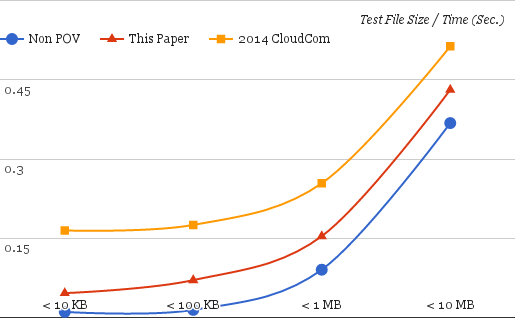
\includegraphics[width=.6\textwidth]{LAB_VM_UP}
    \end{center}
\end{frame}

\begin{frame}{Experimental Results}
{The client device and SP are in the same network segment (UPLOAD)}
	\begin{minipage}[c]{0.4\textwidth}
    \scriptsize
    \begin{table}[] 
    \centering
    \caption{}
    \begin{tabular}{lccc}
        Test File        & Rate     \\ \hline
        \textless 10 KB  & -76.95\% \\ \hline
        \textless 100 KB & -64.97\% \\ \hline
        \textless 1 MB   & -61.24\% \\ \hline
        \textless 10 MB  & -56.68\% \\ \hline
    \end{tabular}
    \end{table}
    \begin{center}
		$Rate\ =\ \frac{(V-N)\ -\ (C-N)}{(C-N)}$
        \begin{equation*} \label{eq3}
                \begin{split}
                        V\ & =\ Voting,\ this\ paper\\
                        C\ & =\ 2014\ Cloud\ Com\\
                        N\ & =\ Non\ POV
                \end{split}
        \end{equation*}
    \end{center}
    \end{minipage}%
    \begin{minipage}[c]{0.6\textwidth}
	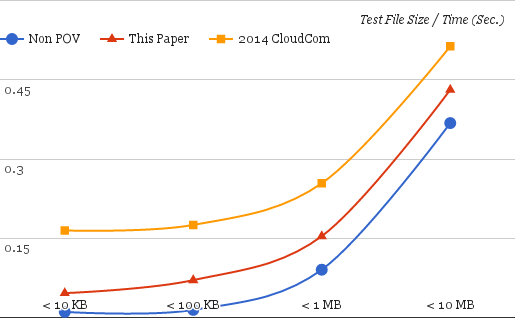
\includegraphics[width=\textwidth]{LAB_VM_UP}
    \end{minipage}
\end{frame}

\begin{frame}{Experimental Results}
{The client device and SP are in the same network segment}
	\scriptsize
    \begin{table}[] 
    \centering
    \caption{THE EXECUTION TIME OF \alert{DOWNLOAD} OPERATIONS (IN SEC.) (Account C)}
    \begin{tabular}{lccc}
        Test File        & Non POV  & This Paper & 2014 CloudCom \\ \hline
        \textless 10 KB  & 0.007845 & 0.042295   & 0.224947      \\ \hline
        \textless 100 KB & 0.013691 & 0.053583   & 0.236347      \\ \hline
        \textless 1 MB   & 0.098570 & 0.146021   & 0.359045      \\ \hline
        \textless 10 MB  & 0.354916 & 0.392072   & 0.961740      \\ \hline
    \end{tabular}
    \end{table}
    \begin{center}
	    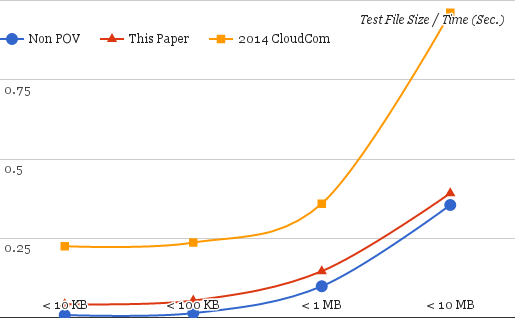
\includegraphics[width=.6\textwidth]{LAB_VM_DO}
    \end{center}
\end{frame}

\begin{frame}{Experimental Results}
{The client device and SP are in the same network segment (DOWNLOAD)}
	\begin{minipage}[c]{0.4\textwidth}
    \scriptsize
    \begin{table}[] 
    \centering
    \caption{}
    \begin{tabular}{lccc}
        Test File        & Rate     \\ \hline
        \textless 10 KB  & -84.13\% \\ \hline
        \textless 100 KB & -82.08\% \\ \hline
        \textless 1 MB   & -81.78\% \\ \hline
        \textless 10 MB  & -93.88\% \\ \hline
    \end{tabular}
    \end{table}
    \begin{center}
		$Rate\ =\ \frac{(V-N)\ -\ (C-N)}{(C-N)}$
        \begin{equation*} \label{eq4}
                \begin{split}
                        V\ & =\ Voting,\ this\ paper\\
                        C\ & =\ 2014\ Cloud\ Com\\
                        N\ & =\ Non\ POV
                \end{split}
        \end{equation*}
    \end{center}
    \end{minipage}%
    \begin{minipage}[c]{0.6\textwidth}
	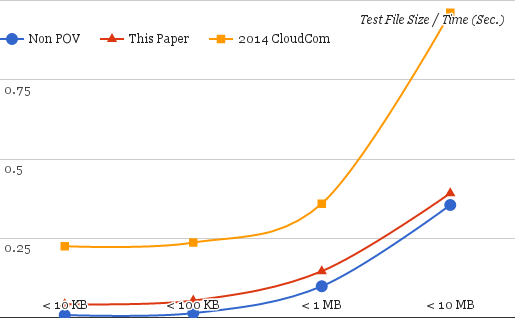
\includegraphics[width=\textwidth]{LAB_VM_DO}
    \end{minipage}
\end{frame}

\begin{frame}{Experimental Results}
{The client device and SP are \alert{not} in the same network segment}
	\scriptsize
	\begin{table}[]  
    \centering
    \caption{THE EXECUTION TIME OF \alert{UPLOAD} OPERATIONS (IN SEC.) (Account C)}
    \begin{tabular}{lccc}
        Test File        & Non POV  & This Paper & 2014 CloudCom \\ \hline
        \textless 10 KB  & 0.077653 & 0.254801   & 0.407407      \\ \hline
        \textless 100 KB & 0.149493 & 0.338238   & 0.492000      \\ \hline
        \textless 1 MB   & 0.631626 & 0.825261   & 0.983832      \\ \hline
        \textless 10 MB  & 4.014217 & 4.182142   & 4.359997      \\ \hline
    \end{tabular}
    \end{table}
	\begin{center}
	    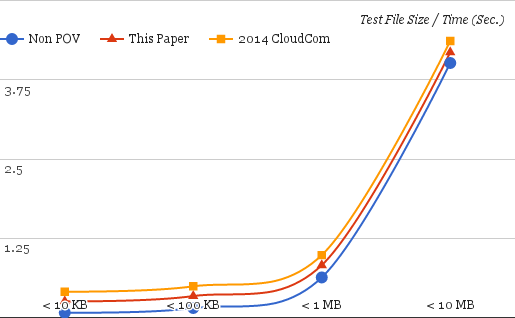
\includegraphics[width=.6\textwidth]{HOME_VM_UP}
    \end{center}
\end{frame}

\begin{frame}{Experimental Results}
{The client device and SP are \alert{not} in the same network segment (UPLOAD)}
	\begin{minipage}[c]{0.4\textwidth}
	\scriptsize
    \begin{table}[] 
    \centering
    \caption{}
    \begin{tabular}{lccc}
        Test File        & Rate     \\ \hline
        \textless 10 KB  & -46.28\% \\ \hline
        \textless 100 KB & -44.89\% \\ \hline
        \textless 1 MB   & -45.02\% \\ \hline
        \textless 10 MB  & -51.44\% \\ \hline
    \end{tabular}
    \end{table}
    \begin{center}
		$Rate\ =\ \frac{(V-N)\ -\ (C-N)}{(C-N)}$
        \begin{equation*} \label{eq5}
                \begin{split}
                        V\ & =\ Voting,\ this\ paper\\
                        C\ & =\ 2014\ Cloud\ Com\\
                        N\ & =\ Non\ POV
                \end{split}
        \end{equation*}
    \end{center}
    \end{minipage}%
    \begin{minipage}[c]{0.6\textwidth}
	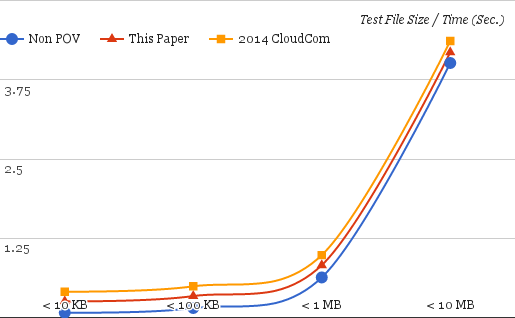
\includegraphics[width=\textwidth]{HOME_VM_UP}
    \end{minipage}
\end{frame}

\begin{frame}{Experimental Results}
{The client device and SP are \alert{not} in the same network segment}
	\scriptsize
    \begin{table}[]
    \centering
    \caption{THE EXECUTION TIME OF \alert{DOWNLOAD} OPERATIONS (IN SEC.) (Account C)}
    \begin{tabular}{lccc}
        Test File        & Non POV  & This Paper & 2014 CloudCom \\ \hline
        \textless 10 KB  & 0.061063 & 0.275808   & 0.538531      \\ \hline
        \textless 100 KB & 0.093941 & 0.312340   & 0.620296      \\ \hline
        \textless 1 MB   & 0.225640 & 0.457329   & 0.752591      \\ \hline
        \textless 10 MB  & 1.147272 & 1.296215   & 1.631534      \\ \hline
    \end{tabular}
    \end{table}
    \begin{center}
	    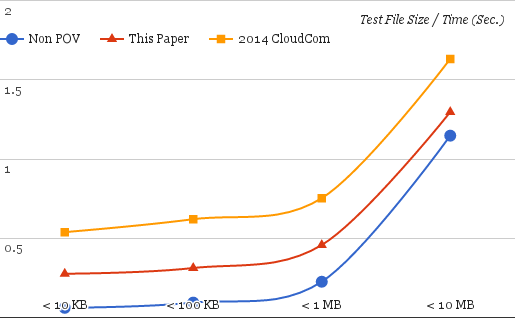
\includegraphics[width=.6\textwidth]{HOME_VM_DO}
    \end{center}
\end{frame}

\begin{frame}{Experimental Results}
{The client device and SP are \alert{not} in the same network segment (DOWNLOAD)}
	\begin{minipage}[c]{0.4\textwidth}
	\scriptsize
    \begin{table}[] 
    \centering
    \caption{}
    \begin{tabular}{lccc}
        Test File        & Rate     \\ \hline
        \textless 10 KB  & -55.02\% \\ \hline
        \textless 100 KB & -58.51\% \\ \hline
        \textless 1 MB   & -56.03\% \\ \hline
        \textless 10 MB  & -69.24\% \\ \hline
    \end{tabular}
    \end{table}
    \begin{center}
		$Rate\ =\ \frac{(V-N)\ -\ (C-N)}{(C-N)}$
        \begin{equation*} \label{eq6}
                \begin{split}
                        V\ & =\ Voting,\ this\ paper\\
                        C\ & =\ 2014\ Cloud\ Com\\
                        N\ & =\ Non\ POV
                \end{split}
        \end{equation*}
    \end{center}
    \end{minipage}%
    \begin{minipage}[c]{0.6\textwidth}
	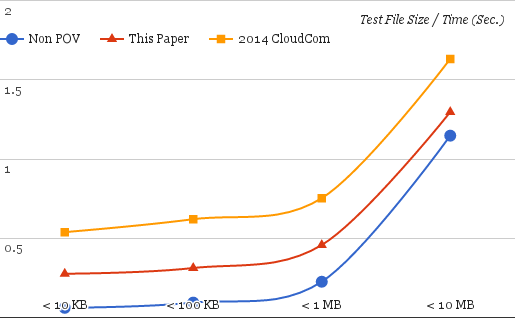
\includegraphics[width=\textwidth]{HOME_VM_DO}
    \end{minipage}
\end{frame}

\begin{frame}{Experimental Results}{Running time of different numbers' servers}
	\scriptsize
	\begin{table}[]
    \centering
    \caption{THE EXECUTION TIME OF \alert{UPLOAD} OPERATIONS (IN SEC.) (Account C)}
    \begin{tabular}{lcccc}
        Test File        & 3 Server & 5 Server & 7 Server & 9 Server \\ \hline
        \textless 10 KB  & 0.046139 & 0.067923 & 0.101676 & 0.108696 \\ \hline
        \textless 100 KB & 0.070739 & 0.083563 & 0.112895 & 0.145049 \\ \hline
        \textless 1 MB   & 0.153822 & 0.166289 & 0.200053 & 0.203870 \\ \hline
        \textless 10 MB  & 0.430937 & 0.513879 & 0.684666 & 0.694259 \\ \hline
    \end{tabular}
    \end{table}
    \begin{center}
	    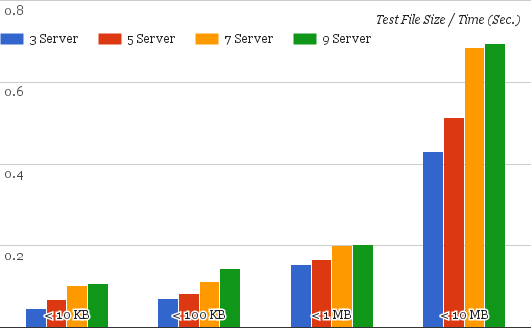
\includegraphics[width=.6\textwidth]{multi_server_UP}
    \end{center}
\end{frame}

\begin{frame}{Experimental Results}{Running time of different numbers' servers}
	\scriptsize
    \begin{table}[]
    \centering
    \caption{THE EXECUTION TIME OF \alert{DOWNLOAD} OPERATIONS (IN SEC.) (Account C)}
    \begin{tabular}{lcccc}
        Test File        & 3 Server & 5 Server & 7 Server & 9 Server \\ \hline
        \textless 10 KB  & 0.042295 & 0.054263 & 0.064370 & 0.078872 \\ \hline
        \textless 100 KB & 0.053583 & 0.055442 & 0.083961 & 0.097507 \\ \hline
        \textless 1 MB   & 0.146021 & 0.159869 & 0.195817 & 0.202213 \\ \hline
        \textless 10 MB  & 0.392072 & 0.476251 & 0.622665 & 0.625499 \\ \hline
    \end{tabular}
    \end{table}
    \begin{center}
	    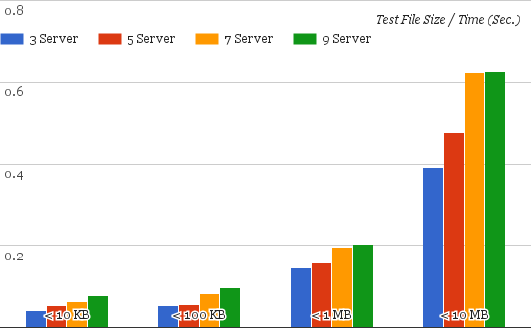
\includegraphics[width=.6\textwidth]{multi_server_DO}
    \end{center}
\end{frame}